\documentclass[compress,xelatex,xcolor=dvipsnames,print]{beamer}
\usecolortheme[named=Brown]{structure}
\usepackage{beamerthemeshadow}
\usepackage{xltxtra}
\usepackage{xunicode}
\usepackage{polyglossia}
\setdefaultlanguage{czech}
\usepackage{multicol}
\author{Vojtěch Zeisek}
\institute{Ekologický odbor Výkonné rady Junáka -- svazu skautů a~skautek ČR\\
Katedra botaniky Přírodovědecké fakulty UK \&~Botanický ústav AV ČR}
\title{Nový výchovný program Junáka}
\subtitle{2005-2013}
\date{KDF MFF UK 27. 3. 2013}
\titlegraphic{\includegraphics[width=2cm]{lilie.png}}

\begin{document}

\begin{frame}
\titlepage
\end{frame}

\section{Úvod}

\begin{frame}{Proč nový program?}
\begin{itemize}
\item Změna dnešní společnosti
 \begin{itemize}
 \item konzumní společnost
 \item zrychlená doba
 \item vliv médií, počítačů, internetu, techniky, \ldots
 \item děti rychleji dospívají a~baví je jiné věci než v~minulosti
 \end{itemize}
\item Konkrétní problémy starého programu
 \begin{itemize}
 \item Mnohé prostředky byly zastaralé a~pro děti neatraktivní
 \item Chybělo jasné stanovení výchovných cílů programu
 \item Postaven převážně na znalostech
 \item Nedostatečná metodická podpora pro vedoucí
 \end{itemize}
\item Historický vývoj Junáka (zákazy, \ldots) a~inspirace v~zahraničí
\item Charta českého skautingu
 \begin{itemize}
 \item Schválena 2005
 \item Odkazuje na historické kořeny, uvědomuje si současný svět a~otevírá skauting pro budoucnost
 \item Obecné cíle rozvoje Junáka
 \end{itemize}
\end{itemize}
\end{frame}

\subsubsection{Výchovný program}

\begin{frame}{Výchovný program}
\begin{itemize}
\item Výsledek skautské výchovy -- výchovné cíle skautingu
 \begin{itemize}
 \item Mladý člověk cca na konci střední až počátku vysoké školy
 \item Dovednosti, schopnosti a~postoje, které má mladý člověk ovládat -- koho chceme vychovat
 \end{itemize}
\item Skautská metoda
\item Věkové kategorie
\item Výchovné nástroje
\item Metodické příručky pro vedoucí
\item Hodnocení kvality oddílu a~výchovného dopadu
\item Management, lidské zdroje, found rising, \ldots
\end{itemize}
\end{frame}

\begin{frame}{Výchovný program}
\begin{itemize}
\item Musí vést k~našim výchovným cílům
\item Musí být v~souladu se skautskými hodnotami
\item Musí dnešní děti bavit
 \begin{itemize}
 \item „Ryby je nutné lovit na to, co chutná rybám a~ne na to, co chutná rybáři.“ (Baden-Powell)
 \end{itemize}
\item Musí být využita skautská výchovná metoda -- osvědčený a~účinný způsob dosahování našich cílů
 \begin{itemize}
 \item Děti v~oddíle průměrně tráví 5~\% svého času. Abychom je mohli pozitivně ovlivnit, musíme tento čas využít maximálně efektivně
 \item Je obecná -- musí dostat konkrétní atraktivní náplň
 \end{itemize}
\end{itemize}
\end{frame}

\begin{frame}{Jak při tvorbě nového výchovného programu postupujeme}
\begin{enumerate}
\item Definování obecných cílů (kompetence)
\item Rozpracování dílčích cílů (podle věku, \ldots)
\item Výběr vhodných indikátorů (jak poznáme, je-li cíl splněn)
\item Tvorba programů vedoucích ke splnění cílů
\end{enumerate}
\begin{itemize}
\item Obecné cíle se definovaly na začátku pro všechny věkové kategorie
\item Rozpracování obecných cílů se provádí pro jednotlivé věkové kategorie
\item Další nástroje sloužící k~motivaci, \ldots
\item Postupná tvorba databáze programů
\item Metodická podpora pro vedoucí a~další „uživatelská“ podpora vedoucím oddílů ze strany organizace
\end{itemize}
\end{frame}

\begin{frame}{Co chceme, aby uměl mladý člověk poté, co projde naší výchovou a~na prahu dospělosti odejde?}
\begin{center}
\includegraphics[height=6.5cm]{pepicek.png}
\end{center}
\end{frame}

\section{Kompetence}

\begin{frame}{Skauting a~klíčové kompetence}
\begin{center}
Klíčové kompetence: přenosný a~univerzálně použitelný \textbf{soubor vědomostí, dovedností a~postojů}, které potřebuje každý jedinec \textbf{pro své osobní naplnění a~rozvoj, pro zapojení se do společnosti} a~úspěšnou zaměstnatelnost.
\end{center}
\begin{itemize}
\item Kompetence je souborem schopností, dovedností, znalostí a~postojů vztahující se k~určité oblasti
\item Kompetence se rovnají výchovným záměrům
\item Jsou rozpracované pro jednotlivé kategorie
\item Navazují na ně výchovné cíle a~metody
\item Úspěšnost definují indikátory (ukazatele, zda dochází k~rozvoji dané kompetence)
\item Jsou zpracovávány a~konzultovány odborníky na danou oblast
\end{itemize}
\end{frame}

\begin{frame}{Poslání Junáka}
\begin{center}
\begin{Large}
Posláním Junáka je \textbf{podporovat rozvoj osobnosti} mladých lidí, jejich \textbf{duchovních, mravních, intelektuálních, sociálních a~tělesných schopností} tak, aby byli po celý život připraveni plnit povinnosti k~sobě samým, bližním, vlasti, přírodě a~celému lidskému společenství \textbf{v~souladu s~principy a~metodami}, stanovenými zakladatelem skautského hnutí, lordem Robertem Baden-Powellem a~zakladatelem českého skautingu, prof. Antonínem Benjamínem Svojsíkem.
\end{Large}
\end{center}
\begin{itemize}
\item Za 1. republiky se na tvorbě skautské metodiky podílely tehdejší špičky psychologie, pedagogiky a~dalších oborů.
\end{itemize}
\end{frame}

\begin{frame}{Skautská výchovná metoda}
\ldots vede mladého člověka na cestě osobního růstu: soustava výchovy a~sebevýchovy vedoucí k~upevňování charakteru, tvorbě hodnotového systému a~rozvoji dovedností a~znalostí.
\begin{itemize}
\item skautský slib a~zákon jako vyjádření životního stylu a~hodnotového systému
\item učení se prostřednictvím praktických činností a~her
\item týmová práce v~malých skupinách (obvykle družinách) rozvíjející spolupráci, vůdčí schopnosti a~odpovědnost za druhé
\item zájem a~spoluúčast každého mladého člověka na jeho osobním rozvoji
\item symbolický rámec nabízející výchovnou motivaci a~inspiraci
\item pobyt a~činnost v~přírodě, její poznávání a~ochrana
\item podpora mladých lidí dospělými a~vzájemná spolupráce
\item služba společnosti
\item postupně stimulující programy
\item využívání skautské symboliky a~výchovného prostředí
\end{itemize}
\end{frame}

\begin{frame}{Principy skautského hnutí}
\begin{enumerate}
\item \textbf{Povinnost k~Bohu}, chápaná jako povinnost hledat v~životě \textbf{vyšší hodnoty než materiální};
 \begin{itemize}
 \item Jde o~morálku, slušnost, dobrotu -- ne nutně o~víru
 \end{itemize}
\item \textbf{povinnost vůči ostatním}, chápaná jako věrnost své vlasti, která je v~souladu s~úsilím o~mír, o~vzájemné pochopení a~spolupráci mezi lidmi, národy a~různými sociálními skupinami; je pojata jako 	\textbf{závazek účastnit se na rozvoji společnosti, jako úcta a~láska prokazovaná bližním a~přírodě};
 \begin{itemize}
 \item Nejsme tu jen sami za sebe, ale jsme součástí širšího společenství, na jehož běhu se chceme aktivně podílet
 \end{itemize}
\item \textbf{povinnost vůči sobě}, chápaná jako odpovědnost za \textbf{rozvoj sebe sama}.
 \begin{itemize}
 \item Nesmíme zapomínat ani na sebe (včetně odpočinku:-)
 \end{itemize}
\end{enumerate}
\end{frame}

\begin{frame}{Seznam kompetencí}
\begin{enumerate}
\item Duchovní kompetence
 \begin{itemize}
 \item Láska, svědomí, meditace, globální zodpovědnost
 \item V~podstatě jde o~morálku v~nejširším smyslu
 \end{itemize}
\item Psychologické (vztahové)
 \begin{itemize}
 \item Já (k~sobě), já a~ty, já a~my, já a~společnost
 \item Sociální dovednosti, začlenění se do společnosti
 \end{itemize}
\item Manažerské
 \begin{itemize}
 \item Sám sobě manažerem, práce s~informacemi a~řešení problému, vlastní názor, odolávání manipulaci, prezentace na veřejnosti, týmová práce, komunikace
 \end{itemize}
\item Občanské (enviromentální)
 \begin{itemize}
 \item Krása -- vnímání a~vytváření, krása a~jedinečnost přírody, vztah k~přírodě, vztah ke krajině, vědomí provázanosti, respekt k~různosti, aktivní občan
 \item Ochrana přírody díky lásce k~ní, aktivní přístup ke světu
 \end{itemize}
\item Praktické dovednosti
 \begin{itemize}
 \item Přežití v~přírodě, osobní dovednosti, společenské dovednosti, řešení krizových situací
 \end{itemize}
\end{enumerate}
\end{frame}

\begin{frame}{Příklad rozpracování jedné kompetence}
\begin{itemize}
\item Kompetence
 \begin{itemize}
 \item Má dovednosti a~nástroje pro praktický život, umí použít „pracovní nástroje“ své doby (politické, finanční, mediální\ldots)
 \end{itemize}
\item Výchovný cíl
 \begin{itemize}
 \item Dokáže hospodařit s~penězi (8-10 let)
 \end{itemize}
\item Metody
 \begin{itemize}
 \item hry, ve kterých jsou použity peníze pro nákup potřebných surovin
 \item nakupování potravin a~jiných věcí pro oddíl
 \item vedení pokladny družiny, vybírání peněz na výpravě
 \end{itemize}
\item Indikátory
\begin{itemize}
 \item šetří si nějaké peníze se svého kapesného
 \item nekupuje si zbytečnosti
 \item bezchybně vrátí peníze po nákupu
\end{itemize}
\end{itemize}
\end{frame}

\subsection{Vazba kompetencí na výchovný program}

\begin{frame}{Vazba výchovných cílů na program}
\begin{itemize}
\item Z~výchovných cílů a~ze skautské metody musí vycházet všechny programové prostředky
\item Členové vedení oddílů musí výchovné cíle znát, musí na ně navazovat program, musí umět s~nimi pracovat
\item Nutno poskytnout dobrou metodiku pro plánování oddílové činnost podle výchovných cílů (ne pouze podle oblastí stezky nebo oblastí skautské praxe)
\item Počítá se se zapojením členů oddílů do výběru z~aktivit sledujících stejný výchovný cíl (tzv. demokratické hry)
\end{itemize}
\end{frame}

\begin{frame}{Oblasti stezky}
\begin{itemize}
\item Moje dovednosti a~znalosti
 \begin{itemize}
 \item Praktický život, fyzická zdatnost, buď připraven, hledání řešení, vyjadřování, zručnost
 \end{itemize}
\item Kdo jsem?
 \begin{itemize}
 \item Já a~můj život, moje svědomí, osobní rozvoj
 \end{itemize}
\item Můj kamarád
 \begin{itemize}
 \item Vztahy mezi lidmi, moje vztahy, komunikace mezi lidmi, pomoc druhým
 \end{itemize}
\item Můj domov
 \begin{itemize}
 \item Moje rodina, moje parta, družina jako tým
 \end{itemize}
\item Svět okolo nás
 \begin{itemize}
 \item Já a~demokracie, já občan, propojený svět, různost světa, příběhy našeho světa
 \end{itemize}
\item Příroda kolem nás
 \begin{itemize}
 \item Pobyt v~přírodě, vnímání přírody, poznávání přírody, hodnota přírody, šetrné chování
 \end{itemize}
\end{itemize}
Smysl užívání kompetencí: \textbf{Proměnit skautské principy v~život}
\end{frame}

\section{Stezka}

\begin{frame}{Stezka pro skautský věk}
Jeden ze základních výchovných nástrojů -- je všestranná, rozličná a~vyžaduje osobní zapojení vedoucích i~dětí
\begin{center}
\includegraphics[height=6cm]{stezka.png}
\end{center}
\end{frame}

\begin{frame}{Stezka nejsou jen 4~sešity}
\begin{multicols}{2}
\begin{itemize}
\item Propracovaný systém nástrojů a~motivačních prvků
\item Prostředek k~dosahování výchovných cílů
\item Hlavní průvodce na cestě osobního rozvoje
\item Motivuje k~osobnímu rozvoji
\item Obsahuje program zajímavý pro dnešní děti
\item Má atraktivní a~srozumitelnou formu
\item Čtyři stupně (věkové kategorie) -- čtyři živly
\end{itemize}
\columnbreak
\includegraphics[height=7cm]{stezky.png}
\end{multicols}
\end{frame}

\begin{frame}{Nováček -- pro začátek}
\begin{multicols}{2}
\begin{itemize}
\item Uvede nováčka do oddílu
\item Zábavná forma
\item Seznámí se skautingem a~vším, co k~němu patří
\item Oddílové doplňky -- variabilní
\item Pro světlušky, vlčata, vodní i~suchozemské skauty a~skautky
\end{itemize}
\columnbreak
\includegraphics[height=7cm]{novacek.png}
\end{multicols}
\end{frame}

\begin{frame}{Postavy a~pomocníci -- plnění je zábava}
\begin{multicols}{2}
\begin{itemize}
\item Symbolický rámec dobrodružného světa
\item Na cestu si dítě jednu z~postav jako průvodce, pomocníka
\item Za každou splněnou oblast získám pomocníka
\item Existuje i~varianta bez fantasy („turistická“) -- oddíl si může vytvořit vlastní symbolický rámec
\end{itemize}
\columnbreak
\includegraphics[height=7cm]{postavy.png}
\end{multicols}
\end{frame}

\begin{frame}{Sacculus}
\begin{multicols}{2}
\begin{itemize}
\item Motivační karetní hra
\item Doplněk ke stezce
\item 9~základních karet a~kamínky
\item 27 speciálních karet pro každý stupeň
\item Za splněný bod stezky 1~speciální karta
\begin{itemize}
 \item Čím více bodů stezky splní, tím silnější je hráč
\end{itemize}
\item V~principu podobné kartám Magic
\end{itemize}
\columnbreak
\includegraphics[height=4cm]{sacculus.png}
\end{multicols}
\end{frame}

\begin{frame}{Nášivky za splnění stupňů stezky -- motivace na začátku}
\begin{itemize}
\item Nášivka na začátku plnění stupně
 \begin{itemize}
 \item Vyjadřuje důvěru, že dítě daný stupeň splní
 \end{itemize}
\item Závěrečný krystal až po splnění všech stupňů
\end{itemize}
\begin{center}
\includegraphics[height=4cm]{kameny.png}
\end{center}
\end{frame}

\begin{frame}{Skautské výzvy -- něco velkého, nevšedního}
\begin{multicols}{2}
\includegraphics[height=6.1cm]{vyzvy.png}
\begin{itemize}
\item Po splnění stupně privilegovaná možnost plnit si jednu výzvu
 \begin{itemize}
 \item Noční bdění
 \item Ranní svítání
 \item Výsadek
 \item Noční návrat
 \item Tři orlí pera
 \item Dva dny bez ničeho
 \item 24 hodin na stromech
 \end{itemize}
\end{itemize}
\end{multicols}
\end{frame}

\begin{frame}{Výhody stezky}
\begin{itemize}
\item Všestrannost, rozličnost a~osobní zapojení
\item Stezka je vodítkem pro vytváření celoročního programu
\item Stezka umožňuje snadné přizpůsobení oddílu
\item Propracovaný nástroj osobního rozvoje
\item Zatraktivnění programu
\end{itemize}
\end{frame}

\begin{frame}{Pravidla a~plnění stezky}
\begin{itemize}
\item Výběr aktivit
 \begin{itemize}
 \item Některé jsou povinné
 \item Vybírá si skaut nebo skautka po konzultaci s~vedoucím (neplní se všechny)
 \item Lze je plnit v~libovolném pořadí
 \item Aktivitu lze upravit, vymyslet
 \end{itemize}
\item kdo hodnotí
 \begin{itemize}
 \item dítě a~dvě další osoby
 \end{itemize}
\item Hodnocení
 \begin{itemize}
 \item Rozdíl 1. a~2. stupeň a~3. a~4.
 \end{itemize}
\item Plnění
 \begin{itemize}
 \item Přímé plnění
 \item Nepřímé plnění
 \item Přímé plnění s~přípravou
 \item Pro některé body nejsou vhodné všechny způsoby
 \end{itemize}
\end{itemize}
\end{frame}

\begin{frame}{Stezka zdaleka není vše\ldots}
\includegraphics[width=\textwidth]{komplet.png}
\end{frame}

\section{Motivace}

\begin{frame}{Co to je motivace?}
\begin{multicols}{2}
\begin{itemize}
\item Bez motivace to v~nevládní neziskové organizaci nejde\ldots~;-)
\item Proč něco děláme?
\item Něco co nás uvede do pohybu\ldots
\item Něco v~nás pracuje a~pohání nás kupředu\ldots
\item Chceme iniciovat chování nebo jednání druhého člověka.
\item Buďme sami motivovaní!
\item Buďme příkladem, ale~buďme to my
\end{itemize}
\columnbreak
\begin{itemize}
\item Co nás motivuje?
 \begin{itemize}
 \item Odměna
 \item Úspěch
 \item Uznání
 \item Povýšení
 \item Osobní růst
 \item Odpovědnost -- Nezklamat ostatní
 \item Být dobrý -- vynikat
 \item Činnost sama -- \textbf{Děti motivuje hlavně to, že~je ta činnost baví!}
 \end{itemize}
\end{itemize}
\end{multicols}
\end{frame}

\begin{frame}{Cíle a~zpětná vazba}
\begin{multicols}{2}
\begin{itemize}
\item Cíl by měl být dostatečně podnětný, ale i~reálný
\item Měl by bát součástí delšího plánu -- obecné (dlouhodobé) a~konkrétní cíle
\item Oddílová činnost musí být zábavná a~motivační, ale musí vést k~plnění výchovných cílů
\end{itemize}
\columnbreak
\begin{itemize}
\item Zpětná vazba by měla být elektivní
\item Je třeba vyzdvihnout, co děti dělají dobře: i~malý pokrok je výhra
\item Co nás čeká a~čeho jsme dosáhli\ldots
\item Vyjádření uznání
 \begin{itemize}
 \item Formálně i~neformálně
 \item Upřímné, nefalšované
 \item Spravedlivá odměna
 \end{itemize}
\end{itemize}
\end{multicols}
\end{frame}

\begin{frame}{Oddílové motivační prostředky}
\begin{itemize}
\item Zapojení do celoroční, táborové hry -- veškerá činnost pak tvoří jeden logický celek
\item Symbolický rámec -- získání zvláštních schopností, \ldots
\item Motivační scénky
\item Bodování
\item Mapa postupu členů v~plnění
\item Speciální odměny všeho druhu
\item Motivace samotným programem
 \begin{itemize}
 \item Program musí být zábavný
 \item Programy lze spojovat do projektů
 \end{itemize}
\item \textbf{Pozor na záměnu prostředku za cíl!}
\end{itemize}
\end{frame}

\section{Závěr}

\begin{frame}{Metodická podpora vedoucích}
\begin{itemize}
\item Web \href{http://krizovatka.skaut.cz/novy-skautsky-program-3/}{http://krizovatka.skaut.cz/novy-skautsky-program-3/}
\item Metodické příručky (za 49 Kč nebo zdarma v~PDF)
\item Semináře (i~na  požádání)
\item Konzultace
\item Přijímáme zpětnou vazbu -- celý proces je lidmi z~oddílů připomínkován a~testován
\end{itemize}
\begin{center}
\includegraphics[width=4cm]{prirucky.png}
\end{center}
\end{frame}

\begin{frame}{Další informace}
\begin{itemize}
\item Informace o~novém skautském výchovném programu: \href{http://krizovatka.skaut.cz/novy-skautsky-program-3/}{http://krizovatka.skaut.cz/novy-skautsky-program-3/}
 \begin{itemize}
 \item Materiály ke stažení
 \item Informace o~seminářích, kurzech, \ldots
 \item Databáze programů
 \item Řada dalších informací\ldots
 \end{itemize}
\item Web pro veřejnost: \href{http://www.skaut.cz/}{http://www.skaut.cz/}
\item Kniha \textbf{Skautské století} (Roman Šantora, Václav Nosek, Slavomil Janov a~Václav Dostál, TDC a~Mladá fronta, 2012), \href{http://www.skaut.cz/knihastoleti}{http://www.skaut.cz/knihastoleti} a~\href{http://www.skautskestoleti.cz/}{http://www.skautskestoleti.cz/}
\item Budete-li mít v~budoucnu dotazy, klidně se mi ozvěte a~zeptejte se: \href{mailto:zeisek@natur.cuni.cz}{zeisek@natur.cuni.cz}, \href{http://trapa.cz/cs/contact}{http://trapa.cz/cs/contact}
\end{itemize}
\end{frame}

\begin{frame}{Děkuji za pozornost\ldots}
\begin{center}
\includegraphics[height=6.5cm]{zaver.jpg}
\end{center}
\begin{flushright}
\begin{large}\ldots otázky?\end{large}
\end{flushright}
\end{frame}

\end{document}